\documentclass[conference,letterpaper]{IEEEtran}
\IEEEoverridecommandlockouts
% The preceding line is only needed to identify funding in the first footnote. If that is unneeded, please comment it out.
\usepackage{cite}
\usepackage{amsmath,amssymb,amsfonts}
\usepackage{algorithmic}
\usepackage{graphicx}
\usepackage{textcomp}
\usepackage{xcolor}
\usepackage{graphicx}               
\usepackage{subfigure}               %插入并排图片
\usepackage{CJK}                     %插入数学公式
\usepackage{indentfirst}             %插入数学公式
\usepackage{amsmath}                 %插入数学公式
\usepackage{upgreek}                 %平方微米单位
\usepackage{tabu}                    %插入表格
\usepackage{booktabs}  
\usepackage{threeparttable}  
\usepackage{multirow} 
\usepackage{multicol} 
\usepackage{arydshln}                %插入表格
\usepackage{makecell}                %加黑某根线
\usepackage{amsmath}
\def\BibTeX{{\rm B\kern-.05em{\sc i\kern-.025em b}\kern-.08em
    T\kern-.1667em\lower.7ex\hbox{E}\kern-.125emX}}
\begin{document}

\title{A Design of Stochastic Circuit With Exact Synthesis\\
\thanks{The work was supported by NSFC under Grant 61871242.}
}

\author{\IEEEauthorblockN{Huiming Tian, and Zhufei Chu$^*$}
\IEEEauthorblockA{EECS, Ningbo University, Ningbo 315211, China \\ $^*$ Email: chuzhufei@nbu.edu.cn}}

\maketitle

\section*{\textbf{Biography}}
The corresponding author Zhufei Chu received the B.S. degree in electronic information science and technology from Shandong University, Weihai, China, in 2008 and the M.S. degree in communication and information system from Ningbo University, Ningbo, China, in 2011, and the Ph.D. degree in the same subject, in 2014. From 2014 to 2017, he is a lecturer at Ningbo University. Now, he holds an Associate Professor position at Ningbo University. During 2016 to 2017, he works as a researcher at the Integrated Systems Laboratory at EPFL, Lausanne, Switzerland in the group of Prof. Giovanni De Micheli. 

\section*{\textbf{Abstract}}
Stochastic computing is an emerging paradigm that converts traditional binary numbers into stochastic bit streams to perform complex arithmetic computing using simple digital circuits. Stochastic circuits are highly fault-tolerant and have been used in many applications.However, due to the large solution space of the problem, the use of heuristics is complex and does not lead to an optimum solution. In this paper, a novel exact synthesis method using Boolean satisfiability (SAT) is proposed to obtain an optimal stochastic circuit, which is a dedicated homogeneous network by using majority-inverter graphs (MIGs) as underlying logic primitives.The experimental results show that the exact synthesis approach produces better circuits, compared with the heuristic approach.  
\vspace{2ex}

\begin{IEEEkeywords}
stochastic computing; exact synthesis; logic synthesis; majority
\end{IEEEkeywords}

\section*{Introduction}
Modern circuit development is limited by a number of constraints, such as voltage variations, thermal variations and soft errors. These physical phenomena are susceptible to errors, so reliability has become an important issue. Stochastic computing has received increasing attention as an unconventional computing method for solving these problems. It is unique in that it represents and processes information in probabilistic form and is highly fault-tolerant for bit flips.Stochastic computation converts numbers $x \in[0,1]$ into stochastic bit streams containing only 0 and 1. The number is represented by the probability of a one in the bit stream. Thus stochastic computing transforms a complex computing unit into a simple  circuit with gate. For example, multiplication in stochastic computing can be implemented with an AND gate, as shown in Fig.1.  Assume
that the two input stochastic bit streams are independent. Stochastic computing has been applied in many applications such as image processing, neural networks, decoding of LDPC, filter design, and so on~\cite{1}.

\begin{figure}[t]
    \setlength{\abovecaptionskip}{0.cm}
    \setlength{\belowcaptionskip}{-0.5cm}
    \centering
    \subfigure{
        \begin{minipage}[t]{1\linewidth}
            \centering
            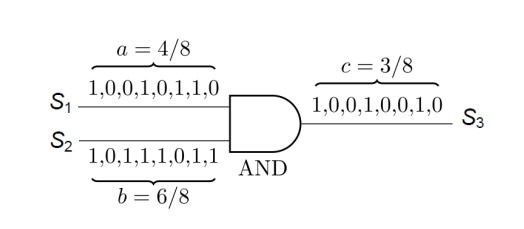
\includegraphics[width=3in]{fig/AND_gate.jpg}
        \end{minipage}
    }
    \caption{AND gate performs multiplication by stochastic bit streams.}
\end{figure}

In stochastic computing, many different Boolean functions can be implemented to compute the same function, which gives great design scope for the synthesis of stochastic circuits. In order to adapt stochastic computing to more functions, researchers have recently proposed several synthesis methods. One of the state-of-the-art methods is a heuristic breadth-first search algorithm~\cite{2},which is based on assigning
cubes (i.e., product terms) to the on-set of the Boolean function. However, heuristics cannot find optimal solutions. Exact synthesis is a new approach, which is a problem of finding logical networks that represent given Boolean functions and respect given constraints. With exact synthesis it is possible to find optimum networks, e.g., in size or depth. In this paper, we use exact synthesis method to obtain an optimal stochastic circuit, which is a dedicated homogeneous network by using MIGs as only logic primitives. The experimental results show that the exact synthesis approach produces better circuits, compared with the heuristic approach.


\section*{Background}
Figure.2 shows a general form of stochastic computing circuit with combination circuit. For a function of single variable x, the stochastic number generator (SNG) generates n inputs $X_{1}, \ldots, X_{n}$, whose probability is x, where n is the highest power of the variable $x$ in the function. SNGs usually consist of a pseudo-random number generator and a comparator.In addition, the linear feedback shift register (LFSR) generates m inputs $Y_{1}, \ldots, Y_{n}$ with probability 0.5. The stochastic bit streams of these n+m inputs are processed by a combination logic circuit.

\begin{figure}[t]
    \setlength{\abovecaptionskip}{0.cm}
    \setlength{\belowcaptionskip}{-0.5cm}
    \centering
    \subfigure{
        \begin{minipage}[t]{1\linewidth}
            \centering
            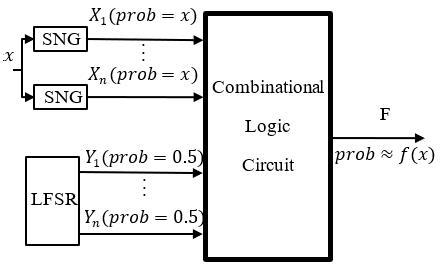
\includegraphics[width=3.3in]{fig/SC6.JPG}
        \end{minipage}
    }
    \caption{A general form of stochastic circuits.}
\end{figure}
As shown in~\cite{2}, the output probability of the circuit in Fig.3 obtains $G(i)$ is the number of minterms $\left(X_{1}, \ldots, X_{n}, Y_{1}, \ldots, Y_{m}\right)$ satisfying that $F\left(X_{1}, \ldots, X_{n}, Y_{1}, \ldots, Y_{m}\right)=1$ and $\sum_{j=1}^{n} X_{j}=i$. $(G(0), \ldots, G(n))$ is recorded as the problem vector. For example, (0, 3, 2) is a problem vector using the 2-dimensional truth table shown in Fig. 3 with $n=2$ and $m=2$.Its output probability realizes the following function:
\begin{equation}
g(x)=\frac{3}{4} x(1-x)+\frac{2}{4} x^{2}
\end{equation}
\begin{figure}
    \setlength{\abovecaptionskip}{0.cm}
    \setlength{\belowcaptionskip}{-0.5cm}
    \centering
    \subfigure{
        \begin{minipage}{1\linewidth}
            \centering
            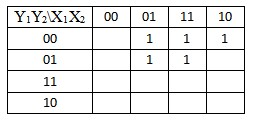
\includegraphics[width=2in]{fig/truth_table.jpg}
        \end{minipage}
    }
    \caption{The truth table of a Boolean function with problem vector (0, 3, 2).}
\end{figure}
The Boolean function shown in Fig. 3 is represented in a simplified sum-of-product (SOP) form:
\begin{equation}
F=X_{2} \overline{Y_{1}}+X_{1} \overline{Y_{1}}     \overline{Y_{2}}
\end{equation}
In this way, the problem vector can form a logical circuit for stochastic computing, but there are many kinds of Boolean functions of the same problem vector. Fig. 3 is just one of the 356 Boolean functions of problem vector (0, 3, 2).

\section*{Proposed Designs}
Exact synthesis is the problem of finding optimal logic networks by giving a set of primitives. The objectives can be the size or logic level of the network, which corresponds to the area and delay
of the circuit, respectively. Based on Boolean satisfiability, exact synthesis is
executed by solving sequences of SAT formulations ~\cite{3}. 
In this section, MIGs are used as underlying logic primitives as their homogeneous logic representation and containing AND/OR-inverter graphs.Majority function with three inputs a, b, and c can be represented as both disjunctive and conjunctive normal forms (CNFs).
\begin{equation}
f=<a b c>=a b \vee a c \vee b c=(a \vee b)(a \vee c)(b \vee c)
\end{equation}

It is well know that the optimal size of a normal network is found via SAT formula. Based on the Knuth algorithm ~\cite{4}, we propose our encoding method about Majority operations. Being $a$, $b$, and $c$ the 3 inputs, each gate can realize $<a b c>$, $<\bar{a} b c>$, $<a \bar{b} c>$ or $<a b \bar{c}>$. By setting any variable to constant 0 or 1, one can behave as AND or OR, respectively. $a b$, $\bar{a} b$, $a \bar{b}$, and $a+b$ should also be considered. The defined variables~\cite{5} are constrained by a set of clauses.For each gate $r$, the operation variable  $o_{r w}$ is true if the operation of gate $r$ is $w$, where $w$ is one of the 8 possible normal majority operations.

For example, suppose the selection variable $S_{i a b c}$, and the input combination is (100), then we can check $o_{r 1}=<abc>$ outputs 0, while $o_{r 8}=a+b$ outputs 1. Thus the clause is added as follows.
%$$ \bar{S}_{i a b c} \vee \bar{x}_{i t} \vee o_{r 3} \vee o_{r 4} \vee o_{r 7} \vee o_{r 8}$$
%$$ \bar{S}_{\text {iabc}} \vee \bar{x}_{i t} \vee \bar{o}_{r 1}$$
%$$\bar{S}_{i a b c} \vee \bar{x}_{i t} \vee \bar{o}_{r 6}$$
%$$\bar{S}_{\text {iabc}} \vee x_{i t} \operatorname{Vo}_{r 1} \operatorname{Vo}_{r 2} \operatorname{Vo}_{r 5} \operatorname{Vo}_{r 6}$$
%$$\bar{S}_{i a b c} \vee x_{i t} \vee \bar{o}_{r 3}$$
%$$\bar{S}_{i a b c} \vee x_{i t} \vee \bar{o}_{r 8}$$
\begin{equation}                     %equations of AU and CU
\begin{split}
&\bar{S}_{i a b c} \vee \bar{x}_{i t} \vee o_{r 3} \vee o_{r 4} \vee o_{r 7} \vee o_{r 8} \\
&\bar{S}_{\text {iabc}} \vee \bar{x}_{i t} \vee \bar{o}_{r 1} \\
&\bar{S}_{\text {iabc}} \vee x_{i t} \vee {o}_{r 1} \vee{o}_{r 2} \vee{o}_{r 5} \vee{o}_{r 6}\\
&\bar{S}_{i a b c} \vee x_{i t} \vee \bar{o}_{r 3}\\
&\bar{S}_{i a b c} \vee x_{i t} \vee \bar{o}_{r 8}\\
\end{split}
\end{equation}

Further, clause $\bigvee_{w=1}^{8} o_{r w}$ ensure that each step should realize at least one of the 8 operations.

Given a problem vector, we use exact synthesis algorithm to find a solution by assuming $r= 1$ gate. If a solution is found, it returns MIG; otherwise, the algorithm will increase the number of gates $r$, then restart encoding and solve until the upper limit is reached. This will ensure that the algorithm can find the MIG network with the best number of gates.

\section*{Experimental Result}
\footnote{https://github.com/nbulsi/also} 


%\bibliographystyle{unsrt}
\bibliography{refs}

\end{document}
